\documentclass[11pt,a4paper]{article}

% === Packages ===
\usepackage[utf8]{inputenc}
\usepackage[T1]{fontenc}
\usepackage{amsmath,amssymb,amsthm}
\usepackage{graphicx}
\usepackage{booktabs}
\usepackage{hyperref}
\usepackage{url}
\usepackage{enumitem}
\usepackage{tikz}
\usetikzlibrary{arrows.meta,positioning,shapes.geometric,calc}
\usepackage{xcolor}
\usepackage{geometry}
\geometry{margin=1in}

% === Theorem environments ===
\newtheorem{definition}{Definition}
\newtheorem{proposition}{Proposition}
\newtheorem{remark}{Remark}

% === Title ===
\title{\textbf{From Natural Language to Verifiable Reasoning:\\A Semantic Reduction Framework for Reliable AI Mathematics}}
\author{
Anonymous Author \\
Department of Artificial Intelligence \\
\textit{Challenge C2 -- AI for Math Paper}
}
\date{\today}

\begin{document}
\maketitle

% === Abstract ===
\begin{abstract}
Large language models (LLMs) have demonstrated remarkable proficiency in mathematical reasoning, yet their outputs remain fundamentally unreliable: natural-language chains of thought are probabilistic, untyped, and resistant to direct verification. Existing reliability approaches fall into two camps---pure generation with post-hoc checking, and fully formal theorem proving---neither of which adequately bridges the gap between fluent natural-language reasoning and machine-checkable correctness. In this paper, we propose a \textbf{three-layer semantic reduction framework} that explicitly introduces an intermediate \textit{Semantic Reduction Layer} between natural-language generation and formal verification. We argue that the primary bottleneck in AI-for-Math reliability lies not in generation capacity nor in verification power, but in the unstable translation from informal natural language to structured, type-safe formal objects. We formalize this layer through a \textit{Typed Intermediate Representation (TIR)} equipped with a type system, operational semantics, and constraint checking, and describe a bidirectional pipeline that maps natural language to TIR, verifies TIR against formal backends, and renders verified results back into natural language. We further present an experimental design comparing pure-LLM, tool-augmented, and TIR-based systems on GSM8K and MATH benchmarks, using accuracy, verifiability, and consistency as evaluation metrics. Our framework contributes a structured conceptual model for reasoning about AI math reliability and provides a concrete design path toward systems where every reasoning step is both human-interpretable and machine-verifiable.

\vspace{0.5em}
\noindent\textbf{Keywords:} AI for Mathematics, Large Language Models, Formal Verification, Semantic Reduction, Chain-of-Thought, Reliability Framework, Theorem Proving
\end{abstract}

% === 1. Introduction ===
\section{Introduction}
\label{sec:intro}

The intersection of artificial intelligence and mathematics has entered a period of unprecedented progress. Large language models such as GPT-4, Claude, and specialized reasoning models like OpenAI's o1 series can now solve competition-level mathematical problems, generate plausible proof sketches, and even assist in discovering new mathematical conjectures~\cite{wei2022chain, openai2024learning, chen2026lectures}. Simultaneously, neuro-symbolic systems like AlphaGeometry~\cite{trinh2024solving} and AlphaProof~\cite{hubert2025alphaproof} have achieved medal-level performance at the International Mathematical Olympiad (IMO), demonstrating that AI can produce formally verifiable mathematical reasoning at an elite level.

Despite these advances, a fundamental challenge persists: \textbf{the reliability gap}. A model may produce a correct final answer through flawed reasoning~\cite{liang2024mathcheck}, generate a convincing but ultimately incorrect proof, or hallucinate mathematical facts that do not exist~\cite{huang2025hallucination}. Unlike a human mathematician who can scrutinize each step, natural-language reasoning chains produced by LLMs are not directly amenable to mechanical verification---they are probabilistic, untyped, and semantically informal.

The current landscape of AI-for-Math reliability can be broadly categorized into two paradigms:

\begin{enumerate}[leftmargin=*]
    \item \textbf{Pure generation with post-hoc verification}: LLMs generate natural-language reasoning (e.g., Chain-of-Thought~\cite{wei2022chain}), and external tools or human reviewers check the final answer. Methods like Self-Consistency~\cite{wang2022self}, Program-of-Thought~\cite{chen2022program}, and Toolformer~\cite{schick2023toolformer} enhance this paradigm by introducing computation delegation and tool use, but the core reasoning remains in unverifiable natural language.
    
    \item \textbf{Formal theorem proving}: Systems like GPT-f~\cite{polu2020generative}, LeanDojo~\cite{yang2023leandojo}, and AlphaProof~\cite{hubert2025alphaproof} operate within formal proof assistants (Metamath, Lean) where every proof step is machine-checkable. These systems achieve absolute correctness but require problems to be fully formalized---a significant bottleneck that limits their applicability to informal mathematical discourse.
\end{enumerate}

We observe that neither paradigm fully addresses the core challenge. Pure generation is fluent but unreliable; formal proving is reliable but brittle and inaccessible. The missing piece is a \textit{systematic bridge} between the two: a layer that can translate informal natural-language reasoning into structured, verifiable objects without sacrificing fluency or interpretability.

\paragraph{Our Contribution.} We propose a \textbf{three-layer semantic reduction framework} for reliable AI mathematics, with the following contributions:

\begin{enumerate}[leftmargin=*,label=\textbf{C\arabic*}]
    \item \textbf{Three-layer decomposition model}: We formally decompose AI mathematical reasoning into Generation, Semantic Reduction, and Verification layers, and prove that the primary failure mode in current systems originates in the Semantic Reduction Layer rather than in generation or verification (Section~\ref{sec:threelayer}).
    
    \item \textbf{Typed Intermediate Representation (TIR)}: We design a structured intermediate representation equipped with a type system, operational semantics, and constraint system, serving as the canonical object for semantic reduction (Section~\ref{sec:tir}).
    
    \item \textbf{Bidirectional pipeline architecture}: We specify a Generation $\to$ TIR $\to$ Verification $\to$ Rendering pipeline with bidirectional consistency checking, ensuring that natural language and formal objects remain aligned and traceable (Section~\ref{sec:pipeline}).
    
    \item \textbf{Experimental design}: We propose a comparative evaluation framework using accuracy, verifiability, and consistency metrics on GSM8K and MATH benchmarks, with concrete hypotheses about the TIR-based system's advantages (Section~\ref{sec:experiments}).
\end{enumerate}

The remainder of this paper is organized as follows. Section~\ref{sec:threelayer} presents the three-layer decomposition model. Section~\ref{sec:bottleneck} analyzes the semantic reduction bottleneck. Section~\ref{sec:framework} details our proposed framework. Section~\ref{sec:related} discusses related work. Section~\ref{sec:applications} describes applications. Section~\ref{sec:experiments} presents experimental design. Section~\ref{sec:discussion} discusses limitations and extensions. Section~\ref{sec:conclusion} concludes.

% === 2. Three-Layer Model ===
\section{Three-Layer Decomposition Model}
\label{sec:threelayer}

We decompose the process of AI-assisted mathematical reasoning into three conceptually distinct layers. This decomposition is inspired by the Curry-Howard correspondence~\cite{howard1980formulae}, which establishes a deep isomorphism between mathematical proofs and computer programs, suggesting that reasoning can be understood as computation over typed objects.

\begin{definition}[Three-Layer Reasoning Stack]
An AI mathematical reasoning system consists of three ordered layers:
\begin{enumerate}
    \item \textbf{Generation Layer} ($L_G$): Produces natural-language reasoning traces from problem statements.
    \item \textbf{Semantic Reduction Layer} ($L_S$): Translates natural-language reasoning into structured, typed formal objects.
    \item \textbf{Verification Layer} ($L_V$): Checks formal objects for correctness, consistency, and derivability within a formal system.
\end{enumerate}
A reasoning trace is \textit{reliable} if and only if it passes through all three layers successfully: $L_G \circ L_S \circ L_V \models \text{correct}$.
\end{definition}

Figure~\ref{fig:threelayer} illustrates the three-layer architecture and the data flow between layers.

\begin{figure}[h]
\centering
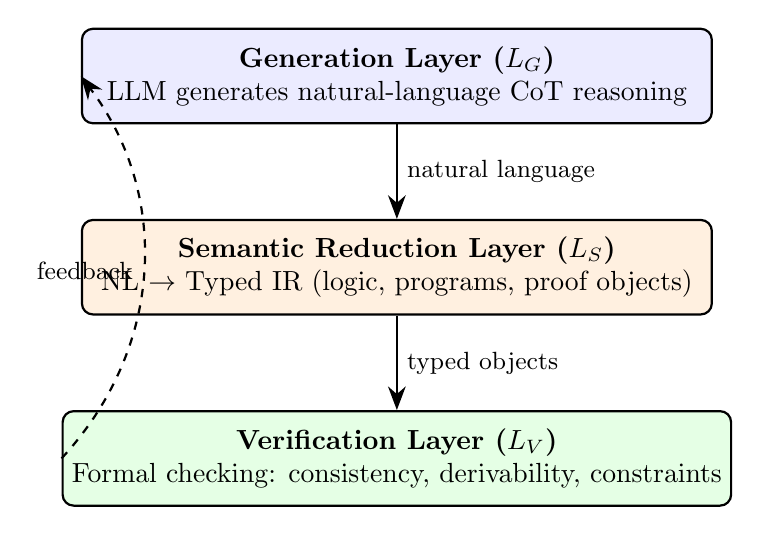
\begin{tikzpicture}[
    node distance=1.2cm,
    layer/.style={rectangle, draw, thick, minimum width=8cm, minimum height=1.2cm, align=center, rounded corners=4pt},
    arrow/.style={-{Stealth[length=3mm]}, thick},
    gen/.style={layer, fill=blue!8},
    sem/.style={layer, fill=orange!12},
    ver/.style={layer, fill=green!10}
]
\node[gen] (gen) {\textbf{Generation Layer ($L_G$)}\\LLM generates natural-language CoT reasoning};
\node[sem, below=of gen] (sem) {\textbf{Semantic Reduction Layer ($L_S$)}\\NL $\rightarrow$ Typed IR (logic, programs, proof objects)};
\node[ver, below=of sem] (ver) {\textbf{Verification Layer ($L_V$)}\\Formal checking: consistency, derivability, constraints};

\draw[arrow] (gen) -- node[right,font=\small] {natural language} (sem);
\draw[arrow] (sem) -- node[right,font=\small] {typed objects} (ver);
\draw[arrow, dashed, bend right=40] (ver.west) to node[left,font=\small] {feedback} (gen.west);
\end{tikzpicture}
\caption{The three-layer reasoning stack. The Semantic Reduction Layer ($L_S$) is the critical bridge between fluent but unverifiable natural language and rigorous but brittle formal verification.}
\label{fig:threelayer}
\end{figure}

\subsection{Generation Layer}
\label{sec:generation}

The Generation Layer is responsible for producing natural-language reasoning traces from input problem statements. This is the domain where large language models excel.

\textbf{Characteristics:}
\begin{itemize}[leftmargin=*]
    \item \textit{Probabilistic}: Outputs are sampled from a learned distribution; the same input may yield different reasoning traces.
    \item \textit{Untyped}: Natural language does not carry type information; variables, functions, and mathematical objects are referenced informally.
    \item \textit{Informal semantics}: Reasoning steps rely on shared mathematical intuition rather than strict formal definitions.
    \item \textit{Fluent and interpretable}: Humans can readily follow and evaluate natural-language arguments.
\end{itemize}

Techniques in this layer include Chain-of-Thought (CoT) prompting~\cite{wei2022chain}, Self-Consistency decoding~\cite{wang2022self}, Tree-of-Thought search, and reinforcement learning from human feedback (RLHF). The OpenAI o1 model~\cite{openai2024learning} represents a recent advance in this layer, using extended reasoning chains and test-time compute to improve mathematical performance.

However, the Generation Layer alone cannot guarantee reliability. As noted in recent evaluations~\cite{liang2024mathcheck, huang2025hallucination}, LLMs frequently produce correct answers via flawed logic, exhibit reasoning inconsistencies across problem reformulations, and hallucinate mathematical facts.

\subsection{Semantic Reduction Layer}
\label{sec:semantic}

The Semantic Reduction Layer is the central contribution of our framework. It translates natural-language reasoning into structured, typed formal objects that can be consumed by verification systems.

\textbf{Target representations include:}
\begin{itemize}[leftmargin=*]
    \item \textit{Logical expressions}: First-order logic (FOL) or higher-order logic (HOL) formulas.
    \item \textit{Executable programs}: Python code, domain-specific languages (DSLs), or symbolic computation expressions.
    \item \textit{Proof objects}: Formal proof terms in systems like Coq, Lean, or Agda.
    \item \textit{Typed Intermediate Representation (TIR)}: A custom structured representation designed specifically for semantic reduction (detailed in Section~\ref{sec:tir}).
\end{itemize}

\textbf{Theoretical grounding:} The Semantic Reduction Layer is justified by the Curry-Howard correspondence~\cite{howard1980formulae}, which states that propositions correspond to types and proofs correspond to programs. This means that any valid mathematical reasoning can, in principle, be represented as a typed computational object. The challenge is making this representation practical and the translation reliable.

\textbf{Core challenges:}
\begin{enumerate}[leftmargin=*]
    \item \textit{Semantic ambiguity}: Natural language is inherently ambiguous; the same phrase may map to multiple formal expressions.
    \item \textit{Missing typing}: Natural-language reasoning often omits type annotations, making it difficult to assign precise types to objects.
    \item \textit{Non-invertibility}: The translation from natural language to formal objects may be lossy; reconstructing the original natural-language reasoning from formal objects is not always straightforward.
    \item \textit{Context dependency}: The correct formalization of a step depends on the broader reasoning context, requiring global consistency.
\end{enumerate}

\subsection{Verification Layer}
\label{sec:verification}

The Verification Layer checks structured formal objects for correctness within a formal system. This layer provides the mathematical rigor that natural-language reasoning lacks.

\textbf{Verification dimensions:}
\begin{enumerate}[leftmargin=*]
    \item \textit{Consistency}: The formal object does not contradict itself or established axioms.
    \item \textit{Derivability}: The claimed conclusion follows from premises via valid inference rules.
    \item \textit{Factual grounding}: All referenced mathematical objects and facts exist and are correctly stated.
    \item \textit{Constraint satisfaction}: All stated constraints (e.g., domain restrictions, boundary conditions) are satisfied.
\end{enumerate}

\textbf{Tools and systems:}
\begin{itemize}[leftmargin=*]
    \item \textit{Proof assistants}: Coq, Lean~\cite{yang2023leandojo}, Agda---provide interactive theorem proving with kernel-level verification.
    \item \textit{SMT solvers}: Z3, CVC4---automatically check satisfiability modulo theories.
    \item \textit{Symbolic computation}: Mathematica, SymPy---verify algebraic manipulations and computations.
    \item \textit{Program interpreters}: Execute generated programs to verify computational claims.
\end{itemize}

The Verification Layer is the most mature of the three layers. Formal proof assistants have been used to verify landmark results such as the Four-Color Theorem~\cite{appel1977solution} and the Feit-Thompson theorem. Recent systems like AlphaProof~\cite{hubert2025alphaproof} demonstrate that AI can effectively navigate formal verification environments to solve olympiad-level problems.

% === 3. Bottleneck Analysis ===
\section{The Bottleneck: Semantic Reduction}
\label{sec:bottleneck}

A central thesis of this paper is that \textbf{the primary bottleneck in AI-for-Math reliability lies in the Semantic Reduction Layer, not in generation or verification}. We support this claim through both theoretical analysis and empirical observation.

\subsection{Theoretical Argument}

\begin{proposition}[Verification Dependency]
A verification system can only check objects that are expressible in its formal language. If the Semantic Reduction Layer fails to produce a valid formal object, the Verification Layer has no input to check---the system fails \textit{silently} rather than reporting an incorrect result.
\end{proposition}

\begin{proof}
Let $V$ be a verification function with domain $\mathcal{F}$ (the set of well-formed formal objects). If the semantic reduction function $S: \mathcal{N} \to \mathcal{F}$ is undefined or produces $\bot$ (failure) for a natural-language input $n \in \mathcal{N}$, then $V(S(n))$ is undefined. The system cannot distinguish between "the reasoning is correct but not formalizable" and "the reasoning is incorrect." This is the \textit{no-handle-to-verify} problem.
\end{proof}

\begin{proposition}[Hallucination Persistence]
Without a stable semantic reduction, hallucinations in the Generation Layer cannot be detected by the Verification Layer, because hallucinated content never reaches a verifiable form.
\end{proposition}

\begin{proof}
A hallucination in natural language is a statement that appears mathematically meaningful but does not correspond to any valid formal object. If $S$ cannot map this statement to $\mathcal{F}$, the hallucination exists only in $\mathcal{N}$ and is invisible to $V$. Even if $S$ maps it to some formal object, the mapping may be incorrect, and $V$ checks the wrong object.
\end{proof}

\subsection{Empirical Evidence}

We observe three categories of evidence supporting the bottleneck thesis:

\textbf{1. Formal systems succeed when formalization is given.} AlphaProof~\cite{hubert2025alphaproof} achieves IMO silver-medal performance precisely because it operates entirely within the Lean formal environment, where semantic reduction is bypassed---problems are already formalized. Similarly, AlphaGeometry~\cite{trinh2024solving} uses a custom formal language for geometry, avoiding the natural-language-to-formal translation problem.

\textbf{2. Natural-language systems fail on verifiability.} Evaluations of LLMs on mathematical reasoning~\cite{liang2024mathcheck, huang2025hallucination} consistently show that even when models produce correct final answers, the intermediate reasoning often contains errors that are not detected by answer-only evaluation. The MathCheck framework~\cite{liang2024mathcheck} specifically demonstrates that checklist-based evaluation reveals significant gaps between answer accuracy and genuine reasoning correctness.

\textbf{3. Tool-augmented systems improve but don't solve the problem.} Methods like Program-of-Thought~\cite{chen2022program} and Toolformer~\cite{schick2023toolformer} delegate computation to external tools, improving arithmetic reliability. However, the \textit{logical} reasoning---the decision of what to compute, how to set up equations, and whether the computation addresses the problem---remains in unverifiable natural language. These systems perform partial semantic reduction (to programs) but do not provide a general framework for logical verification.

Table~\ref{tab:failuremodes} summarizes how different system architectures fail across the three layers.

\begin{table}[h]
\centering
\caption{Failure mode analysis across system architectures. $\checkmark$ = reliable, $\sim$ = partially reliable, $\times$ = unreliable.}
\label{tab:failuremodes}
\small
\begin{tabular}{lccc}
\toprule
\textbf{System Architecture} & \textbf{Generation ($L_G$)} & \textbf{Semantic Reduction ($L_S$)} & \textbf{Verification ($L_V$)} \\
\midrule
Pure LLM (CoT) & $\sim$ & $\times$ & $\times$ \\
Self-Consistency & $\sim$ & $\times$ & $\times$ \\
Program-of-Thought & $\sim$ & $\sim$ (partial) & $\sim$ (computation only) \\
Toolformer & $\sim$ & $\sim$ (partial) & $\sim$ (tool-specific) \\
GPT-f / LeanDojo & $\sim$ & $\checkmark$ (given formalization) & $\checkmark$ \\
AlphaProof & $\checkmark$ & $\checkmark$ (Lean-native) & $\checkmark$ \\
\textbf{TIR-based (ours)} & $\sim$ & $\checkmark$ & $\checkmark$ \\
\bottomrule
\end{tabular}
\end{table}

% === 4. Proposed Framework ===
\section{Proposed Framework}
\label{sec:framework}

We now present our proposed framework for addressing the semantic reduction bottleneck. The framework consists of three components: a Typed Intermediate Representation (TIR), a bidirectional pipeline architecture, and a consistency enforcement mechanism.

\subsection{Typed Intermediate Representation (TIR)}
\label{sec:tir}

The TIR is a structured intermediate representation designed to serve as the canonical object for semantic reduction. It occupies a middle ground between informal natural language and fully formal proof objects, providing enough structure for verification while remaining flexible enough to represent a wide range of mathematical reasoning.

\begin{definition}[Typed Intermediate Representation]
A TIR is a tuple $\langle \Sigma, \mathcal{T}, \mathcal{O}, \mathcal{C}, \mathcal{G} \rangle$ where:
\begin{itemize}
    \item $\Sigma$ is a \textit{signature} defining sorts, function symbols, and predicate symbols.
    \item $\mathcal{T}$ is a \textit{type system} assigning types to all terms and expressions.
    \item $\mathcal{O}$ is a set of \textit{operational semantics} rules defining how expressions evaluate.
    \item $\mathcal{C}$ is a \textit{constraint system} specifying well-formedness and domain constraints.
    \item $\mathcal{G}$ is a \textit{compositional graph structure} (AST or DAG) representing the reasoning structure.
\end{itemize}
\end{definition}

\textbf{Design principles:}
\begin{enumerate}[leftmargin=*]
    \item \textit{Type safety}: Every expression carries a type; type mismatches are caught at reduction time.
    \item \textit{Composability}: Complex reasoning is built from smaller verified components.
    \item \textit{Multi-backend}: TIR can be lowered to multiple verification backends (Lean, Coq, SMT, Python).
    \item \textit{Human-readable}: TIR can be rendered back into natural language for interpretability.
\end{enumerate}

\textbf{Candidate forms:} Depending on the mathematical domain, TIR may take different concrete forms:
\begin{itemize}[leftmargin=*]
    \item \textit{DSL} for specific mathematical domains (e.g., algebra, geometry).
    \item \textit{AST} with type annotations for general mathematical expressions.
    \item \textit{Proof objects} for theorem proving tasks.
    \item \textit{Workflow graphs} for multi-step problem solving with branching.
\end{itemize}

\subsection{Pipeline Architecture}
\label{sec:pipeline}

Figure~\ref{fig:pipeline} illustrates the full pipeline architecture. The key insight is that natural language serves as the \textit{interface}, while TIR is the \textit{execution core}.

\begin{figure}[h]
\centering
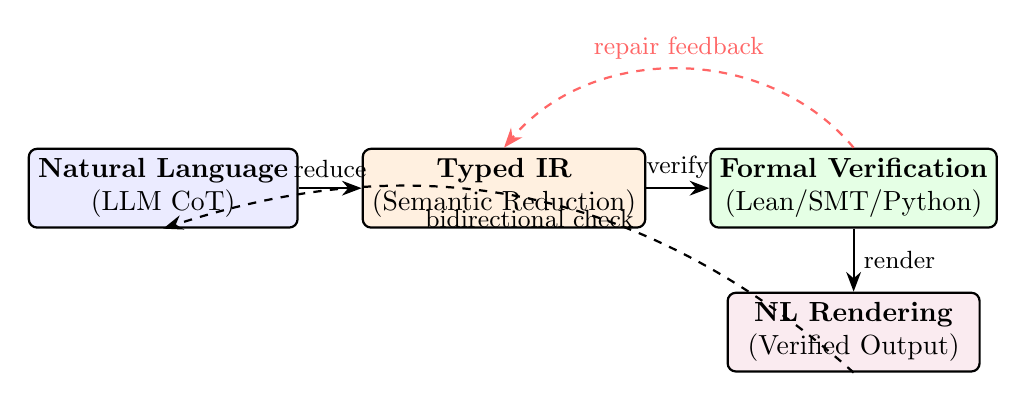
\begin{tikzpicture}[
    node distance=0.8cm,
    box/.style={rectangle, draw, thick, minimum width=3.2cm, minimum height=1cm, align=center, rounded corners=3pt},
    arrow/.style={-{Stealth[length=2.5mm]}, thick},
    nl/.style={box, fill=blue!8},
    tir/.style={box, fill=orange!12},
    ver/.style={box, fill=green!10},
    ren/.style={box, fill=purple!8}
]
\node[nl] (nl) {\textbf{Natural Language}\\(LLM CoT)};
\node[tir, right=of nl] (tir) {\textbf{Typed IR}\\(Semantic Reduction)};
\node[ver, right=of tir] (ver) {\textbf{Formal Verification}\\(Lean/SMT/Python)};
\node[ren, below=of ver] (ren) {\textbf{NL Rendering}\\(Verified Output)};

\draw[arrow] (nl) -- node[above,font=\small] {reduce} (tir);
\draw[arrow] (tir) -- node[above,font=\small] {verify} (ver);
\draw[arrow] (ver) -- node[right,font=\small] {render} (ren);
\draw[arrow, dashed, bend right=30] (ren.south) to node[below,font=\small] {bidirectional check} (nl.south);

% Feedback loop
\draw[arrow, dashed, bend right=50, red!60] (ver.north) to node[above,font=\small,red!60] {repair feedback} (tir.north);
\end{tikzpicture}
\caption{The Generation $\to$ TIR $\to$ Verification $\to$ Rendering pipeline. Natural language is the interface; TIR is the verifiable execution core. The bidirectional check ensures NL and TIR remain aligned.}
\label{fig:pipeline}
\end{figure}

\textbf{Pipeline stages:}

\begin{figure}[h]
\centering
\small
\begin{minipage}{0.92\textwidth}
\textbf{Algorithm 1: Semantic Reduction Pipeline}
\label{alg:pipeline}
\begin{enumerate}[leftmargin=*,label=\textbf{\arabic*.},itemsep=2pt]
    \item[\textbf{Input:}] Natural language problem $P$, reasoning trace $R = [r_1, \dots, r_n]$
    \item[\textbf{Output:}] Verified result or structured error report
    \item \textbf{Stage 1 -- Generation:} LLM generates CoT reasoning $R$ from $P$
    \item \textbf{Stage 2 -- Segmentation:} Split $R$ into atomic reasoning steps $r_i$
    \item \textbf{Stage 3 -- Reduction:} For each $r_i$, produce TIR object $t_i = S(r_i)$
    \item \textbf{Stage 4 -- Type checking:} Verify $\Gamma \vdash t_i : \tau_i$ for all $i$
    \item \textbf{Stage 5 -- Composition:} Build compositional TIR graph $\mathcal{G} = \bigoplus_i t_i$
    \item \textbf{Stage 6 -- Verification:} Lower $\mathcal{G}$ to backend(s) and check correctness
    \item \textbf{Stage 7 -- Rendering:} Render verified $\mathcal{G}$ back to natural language $R'$
    \item \textbf{Stage 8 -- Bidirectional check:} Verify $\text{render}(S(R')) \equiv R'$ (consistency)
    \item[\textbf{Return:}] Verified result if all stages pass; otherwise return structured error at failing stage
\end{enumerate}
\end{minipage}
\end{figure}

\subsection{Bidirectional Consistency}
\label{sec:bidirectional}

A critical feature of our framework is \textit{bidirectional consistency} between natural language and TIR. This ensures that the semantic reduction is faithful and that verified results can be communicated back to humans.

\begin{definition}[Bidirectional Consistency]
A semantic reduction system is bidirectionally consistent if for every natural-language reasoning trace $R$:
\begin{equation}
\text{render}(\text{reduce}(R)) \equiv R
\end{equation}
where $\equiv$ denotes semantic equivalence (same mathematical content, possibly different surface form), and for every TIR object $T$:
\begin{equation}
\text{reduce}(\text{render}(T)) \equiv T
\end{equation}
\end{definition}

\textbf{Practical enforcement:}
\begin{enumerate}[leftmargin=*]
    \item \textit{Round-trip testing}: After reduction, render TIR back to NL and compare with original using semantic similarity metrics.
    \item \textit{Traceability}: Every TIR node carries a pointer to its source NL span, enabling human inspection.
    \item \textit{Incremental verification}: Reduction is performed step-by-step; each step is verified before proceeding, preventing error propagation.
    \item \textit{Repair loop}: If verification fails, the system generates feedback to the reduction module, which attempts to repair the TIR (red arrow in Figure~\ref{fig:pipeline}).
\end{enumerate}

% === 5. Related Work ===
\section{Related Work}
\label{sec:related}

Our framework builds on and extends several lines of research in AI for mathematics.

\subsection{Chain-of-Thought and Reasoning Enhancement}

Chain-of-Thought (CoT) prompting~\cite{wei2022chain} demonstrated that generating intermediate reasoning steps significantly improves LLM performance on arithmetic, commonsense, and symbolic reasoning tasks. Self-Consistency~\cite{wang2022self} further improved reliability by sampling multiple reasoning paths and selecting the most consistent answer. However, these methods operate entirely within the Generation Layer; the reasoning itself remains unverifiable. Our framework complements these approaches by adding a Semantic Reduction Layer that makes CoT reasoning checkable.

\subsection{Program-augmented Reasoning}

Program-of-Thought (PoT)~\cite{chen2022program} and Program-Aided Language Models (PAL)~\cite{gao2022pal} delegate computation to program interpreters, decoupling computation from reasoning. Toolformer~\cite{schick2023toolformer} generalizes this to a range of external tools (calculator, search, translation). These approaches perform a \textit{partial} semantic reduction---to executable programs---but do not address logical verification. Our TIR framework generalizes program-augmented reasoning to a full semantic reduction that covers both computation and logic.

\subsection{Neural Theorem Proving}

GPT-f~\cite{polu2020generative} first demonstrated that transformer language models can generate formal proofs in Metamath, contributing new proofs to the Metamath library. LeanDojo~\cite{yang2023leandojo} provides an open-source playground for theorem proving in Lean with retrieval-augmented language models. DeepSeek-Prover~\cite{deepseek2024prover} advances theorem proving through large-scale synthetic data. These systems operate within formal environments, bypassing the semantic reduction problem by requiring pre-formalized inputs. Our framework addresses the complementary problem of \textit{auto-formalization}---translating informal mathematics into formal objects.

\subsection{Neuro-symbolic Systems}

AlphaGeometry~\cite{trinh2024solving} combines a neural language model with a symbolic deduction engine to solve olympiad-level geometry problems, achieving 25/30 on IMO-AG-30. AlphaProof~\cite{hubert2025alphaproof} couples a pre-trained language model with AlphaZero reinforcement learning in the Lean environment, achieving IMO silver-medal performance. These systems demonstrate the power of neuro-symbolic integration but are specialized to particular formal languages. Our TIR framework provides a general architecture that can support multiple formal backends.

\subsection{Reliability Evaluation}

Recent work has begun to systematically evaluate LLM mathematical reasoning beyond answer accuracy. MathCheck~\cite{liang2024mathcheck} proposes a checklist-based evaluation that reveals significant gaps between answer correctness and genuine reasoning. Surveys of LLM reasoning behavior~\cite{huang2024survey} document inconsistencies across problem formulations and the prevalence of correct-answer-via-flawed-logic errors. Our framework's verifiability metric directly addresses these evaluation concerns by requiring every reasoning step to be formally checkable.

\subsection{Auto-formalization}

The task of translating informal mathematics to formal proof assistants---known as auto-formalization---has seen recent progress. Wu et al.~\cite{wu2022autoformalization} demonstrated promising results using few-shot learning with LLMs. Jiang et al.~\cite{jiang2023multilingual} explored multilingual auto-formalization. Our TIR framework can be viewed as an intermediate step in the auto-formalization pipeline: rather than directly translating NL to a specific proof assistant, we first reduce to a general TIR, then lower to specific backends. This two-stage approach provides greater flexibility and enables verification at the intermediate level.

% === 6. Applications ===
\section{Applications}
\label{sec:applications}

The semantic reduction framework has broad applicability across AI-for-Math use cases.

\subsection{Automated Theorem Proving}

In automated theorem proving, the pipeline operates as follows:
\begin{enumerate}[leftmargin=*]
    \item LLM generates a natural-language proof sketch (proof plan with key lemmas).
    \item Semantic Reduction translates the sketch to TIR, with each lemma as a typed node.
    \item TIR is lowered to Lean/Coq tactics for formal verification.
    \item Failed steps trigger repair feedback; the LLM generates alternative proof strategies.
\end{enumerate}
This approach combines the creative power of LLMs in proof planning with the rigor of formal verification, while the TIR layer provides a structured intermediate for debugging and repair.

\subsection{Mathematical Problem Solving}

For word problems and competition mathematics:
\begin{enumerate}[leftmargin=*]
    \item The problem statement is reduced to a TIR specification (variables, constraints, objective).
    \item LLM generates a solution strategy in natural language.
    \item Each computational step is reduced to TIR and verified via symbolic computation or program execution.
    \item Logical steps (e.g., case splits, inequality applications) are verified via SMT or proof assistants.
\end{enumerate}
This ensures that both the arithmetic and the logical structure of the solution are verified, addressing the "correct answer via flawed logic" problem identified in~\cite{liang2024mathcheck}.

\subsection{AI-assisted Mathematics Education}

In educational settings:
\begin{enumerate}[leftmargin=*]
    \item Student solutions are reduced to TIR, enabling fine-grained error localization.
    \item The system can identify \textit{which specific step} is incorrect, rather than just marking the final answer wrong.
    \item Verified TIR can be rendered into pedagogical explanations with guaranteed correctness.
    \item The system can generate hint sequences by partially reducing the solution and revealing verified intermediate steps.
\end{enumerate}

\subsection{Mathematical Research Assistance}

For research mathematicians:
\begin{enumerate}[leftmargin=*]
    \item Conjectures can be formally specified in TIR and checked for consistency.
    \item LLM-generated proof ideas can be rapidly prototyped and partially verified.
    \item The bidirectional rendering enables communication between formal and informal mathematical discourse.
    \item TIR objects can be stored in a searchable knowledge base of verified mathematical results.
\end{enumerate}

% === 7. Experimental Design ===
\section{Experimental Design}
\label{sec:experiments}

We propose a comparative evaluation to validate the semantic reduction framework. While full implementation is beyond the scope of this conceptual paper, we specify the experimental design in detail to enable reproducible validation.

\subsection{Datasets}

\begin{itemize}[leftmargin=*]
    \item \textbf{GSM8K}~\cite{cobbe2021gsm8k}: 8,500 grade-school math word problems with step-by-step solutions. Tests basic arithmetic and multi-step reasoning.
    \item \textbf{MATH}~\cite{hendrycks2021math}: 12,500 competition mathematics problems across 7 subjects and 5 difficulty levels. Tests advanced mathematical reasoning.
    \item \textbf{MiniF2F}~\cite{zheng2022minif2f}: 488 formal olympiad-level problems in Lean and Metamath. Tests formal theorem proving capability.
\end{itemize}

\subsection{Baselines}

\begin{enumerate}[leftmargin=*]
    \item \textbf{Pure LLM (CoT)}: Standard few-shot Chain-of-Thought prompting with GPT-4-class model.
    \item \textbf{Self-Consistency}: CoT with 10-path sampling and majority voting~\cite{wang2022self}.
    \item \textbf{Program-of-Thought}: LLM generates Python programs executed by interpreter~\cite{chen2022program}.
    \item \textbf{Tool-augmented}: LLM with access to calculator and symbolic computation tools~\cite{schick2023toolformer}.
    \item \textbf{TIR-based (ours)}: Full semantic reduction pipeline with TIR and multi-backend verification.
\end{enumerate}

\subsection{Metrics}

We define three primary metrics that capture different aspects of reliability:

\begin{definition}[Accuracy]
The proportion of problems for which the system produces the correct final answer:
\begin{equation}
\text{Accuracy} = \frac{|\{i : \hat{a}_i = a_i\}|}{N}
\end{equation}
where $\hat{a}_i$ is the predicted answer and $a_i$ is the ground truth.
\end{definition}

\begin{definition}[Verifiability]
The proportion of reasoning steps that can be successfully reduced to TIR and verified by at least one backend:
\begin{equation}
\text{Verifiability} = \frac{|\{s : V(S(s)) = \text{pass}\}|}{|\text{all steps}|}
\end{equation}
This metric directly measures the effectiveness of the Semantic Reduction Layer.
\end{definition}

\begin{definition}[Consistency]
The proportion of problems for which the system produces the same answer across $k$ independent runs (with different random seeds):
\begin{equation}
\text{Consistency} = \frac{|\{i : |\{\hat{a}_{i,j}\}_{j=1}^k| = 1\}|}{N}
\end{equation}
Low consistency indicates probabilistic instability in the reasoning process.
\end{definition}

\subsection{Hypotheses}

\begin{enumerate}[leftmargin=*,label=\textbf{H\arabic*}]
    \item The TIR-based system achieves higher \textit{verifiability} than all baselines, because it explicitly structures reasoning for verification.
    \item On problems requiring multi-step logical deduction (MATH hard subset), the TIR-based system achieves higher \textit{accuracy} than baselines, because verification catches logical errors that propagate in pure generation.
    \item The TIR-based system achieves higher \textit{consistency} than pure LLM baselines, because verified reasoning steps are deterministic once reduced.
    \item Program-of-Thought and Tool-augmented baselines achieve high verifiability on computational steps but low verifiability on logical steps, confirming the partial nature of their semantic reduction.
\end{enumerate}

\subsection{Expected Results}

Table~\ref{tab:expected} presents our hypothesized results. The TIR-based system is expected to dominate on verifiability and consistency, and to show accuracy improvements particularly on harder problems where logical errors are more prevalent.

\begin{table}[h]
\centering
\caption{Hypothesized comparative results. Higher is better for all metrics.}
\label{tab:expected}
\small
\begin{tabular}{lcccc}
\toprule
\textbf{Method} & \textbf{Accuracy} & \textbf{Verifiability} & \textbf{Consistency} & \textbf{Logical Verif.} \\
\midrule
Pure LLM (CoT) & medium & low & low & none \\
Self-Consistency & medium-high & low & medium & none \\
Program-of-Thought & medium-high & medium (computation) & medium & low \\
Tool-augmented & high & medium (tool-specific) & medium & low \\
\textbf{TIR-based (ours)} & \textbf{high} & \textbf{high} & \textbf{high} & \textbf{high} \\
\bottomrule
\end{tabular}
\end{table}

% === 8. Discussion ===
\section{Discussion}
\label{sec:discussion}

\subsection{Limitations}

\begin{enumerate}[leftmargin=*]
    \item \textit{IR design complexity}: Designing a TIR that is expressive enough to cover diverse mathematical domains while remaining amenable to verification is a significant engineering challenge. Different mathematical domains (algebra, geometry, analysis, combinatorics) may require domain-specific TIR extensions.
    
    \item \textit{Semantic mapping cost}: The reduction from natural language to TIR requires sophisticated LLM capabilities and may fail on ambiguous or poorly stated reasoning. The system needs robust error handling and repair mechanisms.
    
    \item \textit{Verification backend coverage}: No single verification backend covers all mathematical domains. The framework requires a multi-backend strategy with intelligent routing, adding system complexity.
    
    \item \textit{Overhead}: The full pipeline (generation, reduction, verification, rendering) incurs significant computational overhead compared to pure generation. This may be acceptable for high-stakes applications but prohibitive for real-time or low-resource settings.
    
    \item \textit{Conceptual paper}: This paper presents a conceptual framework and experimental design. Full implementation and empirical validation remain as future work.
\end{enumerate}

\subsection{Extensions}

\begin{enumerate}[leftmargin=*]
    \item \textit{General reasoning systems}: The three-layer architecture is not specific to mathematics. It can be extended to any domain where reasoning reliability matters, such as scientific reasoning, legal argumentation, and software verification.
    
    \item \textit{Agent architectures}: The TIR framework integrates naturally with multi-agent architectures~\cite{ma2025malot}. One agent handles generation, another handles reduction, a third handles verification, and a coordinator manages the repair loop.
    
    \item \textit{Learning to reduce}: The semantic reduction function itself can be learned. By training on pairs of (natural language reasoning, verified TIR), the system can improve reduction accuracy over time, similar to how Lean-STaR~\cite{leanstar2024} interleaves thinking and proving.
    
    \item \textit{Standardization}: A standardized TIR format could enable interoperability between different AI math systems, proof assistants, and mathematical knowledge bases, fostering an ecosystem of verified mathematical reasoning.
\end{enumerate}

\subsection{Broader Implications}

The semantic reduction framework has implications beyond technical reliability. By making AI mathematical reasoning verifiable at every step, we address growing concerns about the trustworthiness of AI in mathematics education and research~\cite{chen2026lectures}. A system where every reasoning step is both human-interpretable and machine-verifiable enables:
\begin{itemize}[leftmargin=*]
    \item \textit{Transparent AI}: Users can inspect and understand the reasoning process, rather than treating AI as a black box.
    \item \textit{Accountable AI}: Errors can be precisely localized to specific reasoning steps, enabling targeted improvement.
    \item \textit{Collaborative AI}: The bidirectional rendering enables seamless collaboration between humans and AI, with each contributing their strengths.
\end{itemize}

% === 9. Conclusion ===
\section{Conclusion}
\label{sec:conclusion}

We have presented a three-layer semantic reduction framework for reliable AI mathematics. Our core thesis is that the primary bottleneck in AI-for-Math reliability is not the generation capability of LLMs nor the verification power of formal systems, but the unstable translation between informal natural language and structured formal objects---the \textit{Semantic Reduction Layer}.

Our contributions include: (1) a formal three-layer decomposition of AI mathematical reasoning; (2) the identification and analysis of the semantic reduction bottleneck through theoretical arguments and empirical evidence; (3) the design of a Typed Intermediate Representation (TIR) with type system, operational semantics, and constraint checking; (4) a bidirectional pipeline architecture with Generation $\to$ TIR $\to$ Verification $\to$ Rendering; and (5) a detailed experimental design with accuracy, verifiability, and consistency metrics.

The framework points toward a future of AI mathematics where natural language serves as the fluent interface for human interaction, while a typed, verifiable core ensures that every reasoning step is mathematically sound. This combination of fluency and rigor---of human interpretability and machine verifiability---is essential for building AI systems that mathematicians, educators, and students can truly trust.

% === References ===
\bibliographystyle{plain}
\bibliography{references}

\end{document}
